\subsection{导数}

首先,我们来讨论一下函数的极限和连续性问题.
\begin{definition}
    设$w=f(z)$在$z_0$的邻域有定义,对于任意
$\epsilon > 0$,存在$\delta > 0$,使得$|z-z_0| < \delta$时,有
\begin{equation}
    |f(z) - w_0| < \delta ,
\end{equation}
称$z\to z_0$时$w_0$为$f(z)$的{\bf 极限},记为
\begin{equation}
    \lim_{z\to z_0} f(z) = w_0 .
\end{equation}
\end{definition}
当$z$以任意方式趋近$z_0$时都有$ \lim_{z\to z_0} f(z) = w_0$,称$f(z)$在$z_0$点{\bf 连续}.
如果$f(z)$ 在$z_0=x_0 + \imath y_0$点连续,可以等价为
\begin{align}
    \lim_{\substack{x\to x_0\\y\to y_0}} \left(u(x,y), v(x,y)\right) = \left(u(x_0, y_0), v(x_0, y_0)\right) . 
\end{align}

复变函数的导数定义同实函数一样,定义为
\begin{align}
    \label{eq:derivative_def}
    f'(z) = \frac{df}{dz} 
    \equiv\lim_{\Delta z \to 0} \frac{\Delta w} {\Delta z} 
    = \lim_{\Delta z\to 0} \frac{f(z+\Delta z) - f(z) } {(z+\Delta z ) - z}
\end{align}
这里的前提条件是该极限与$\Delta z \to 0$的方式无关.该极限为函数$f(z)$在$z$点的导数.通过该定义,实函数的求导公式对于复变函数同样试用,如
$(f+g)' = f' + g', (fg)' =f'g + fg'$等.与实变函数求导不同的是,复变函数导数存在条件是$\Delta z$以任意方式趋于$0$,因而可导条件的要求比较严格.

\begin{figure}
    \centering
    \begin{tikzpicture}[scale=3]
    \draw[->] (-0.2,0) -- (1.2,0) node[right] {$\operatorname{Re}(z)$};
    \draw[->] (0,-0.2) -- (0,1.0) node[above] {$\operatorname{Im}(z)$};
    % \draw[dashed] (0.5,-1.5) -- (0.5,1.5);
    % \draw[dashed] (-1.5,0.5) -- (1.5,0.5);
    \draw[-latex] (1.0,0.3) -- (1.0,0.8) node[midway, right] {$\substack{\delta y\to 0\\\delta x=0}$};
    \draw[-latex] (0.3,0.8) -- (1.0,0.8) node[midway, above] {$\substack{\delta x\to 0\\\delta y=0}$};
    \filldraw [fill=none] (1,0.8) circle (0.02) node[above right] {$z_0$};
    \node at (0,0) [below left] {$O$};
\end{tikzpicture}
    \caption{逼近$z_0$的两种特殊方式.}
    \label{fig:limits}
\end{figure}
按照图\eqref{fig:limits})两种方式逼近$z_0$,可以得到
\begin{align}
    \lim _{\Delta z \rightarrow 0} \frac{\Delta f}{\Delta z} &=\lim _{\Delta x \rightarrow 0}\left(\frac{\Delta u}{\Delta x}+i \frac{\Delta v}{\Delta x}\right)=\frac{\partial u}{\partial x}+i \frac{\partial v}{\partial x},
\\
    \lim _{\Delta z \rightarrow 0} \frac{\Delta f}{\Delta z} &=\lim _{\Delta y \rightarrow 0}\left(-i \frac{\Delta u}{\Delta y}+\frac{\Delta v}{\Delta y}\right)=-i \frac{\partial u}{\partial y}+\frac{\partial v}{\partial y}
\end{align}
于是,令实部虚部分别相等,即
\begin{equation}
    \begin{cases}
        \frac{\partial u}{\partial x}=\frac{\partial v}{\partial y} \\
        \frac{\partial v}{\partial x}=-\frac{\partial u}{\partial y} .
    \end{cases}
\end{equation}
这就是著名的{\bf 柯西-黎曼条件}(Cauchy-Riemann conditions)或{\bf 柯西-黎曼方程},是复变函数可导的必要条件,但不是充分条件.
% \begin{equation}
%     \left\{\begin{array}{l}
%     \frac{\partial u}{\partial x}=\frac{\partial v}{\partial y} \\
%     \frac{\partial v}{\partial x}=-\frac{\partial u}{\partial y}
%     \end{array}\right.
% \end{equation}
下面我们证明:若$u(x,y), v(x,y)$偏微分存在且连续,并满足柯西-黎曼条件,则$f(z)$可导.
\begin{proof}
    由于$u,v$偏微分连续,可得
    \[
        \Delta f=\left(\frac{\partial u}{\partial x}+\imath \frac{\partial v}{\partial x}\right) \Delta x+\left(\frac{\partial u}{\partial y}+ \imath \frac{\partial v}{\partial y}\right) \Delta y
    \]
    利用柯西-黎曼方程,将上式转换为
    \[
        \begin{aligned}
        \Delta f & =\left(\frac{\partial u}{\partial x}+ \imath \frac{\partial v}{\partial x}\right) \Delta x+\left(-\frac{\partial v}{\partial x}+ \imath\frac{\partial u}{\partial x}\right) \Delta y \\
        & =\left(\frac{\partial u}{\partial x}+ \imath \frac{\partial v}{\partial x}\right)(\Delta x+ \imath \Delta y) 
        \\
        & = \left(\frac{\partial u}{\partial x}+ \imath \frac{\partial v}{\partial x}\right) \Delta z
        \end{aligned}
    \]
可以看到右式与$\Delta z\to 0$的方式无关,因此根据可导的定义判断$f(z)$可导.
\end{proof}
对于极坐标系,我们也可以得到相应的柯西-黎曼方程,
\begin{equation}
    \left\{\begin{array}{l}
    \frac{\partial u}{\partial \rho}=\frac{1}{\rho} \frac{\partial v}{\partial \varphi} \\
    \frac{1}{\rho} \frac{\partial u}{\partial \varphi}=-\frac{\partial v}{\partial \rho}
    \end{array}\right.
    \end{equation}
其中两种推导作为习题.